\section{Adaptation of TFHE and the \texttt{tfhe-rs} Library}
\label{sec:TFHE_adaptation}

From a high level point of view, our technique can be seen as adding an additional layer of abstraction on top of TFHE. However things are not that simple: picking odd values for $p$ leads to some changes in the inner working of the programmable bootstrapping (PBS), and the choice of parameters is also affected by this change. Moreover, we implemented our framework by forking the \texttt{tfhe-rs} library~\cite{tfhe-rs} written in Rust. The following section covers the adaptation of the PBS and the choice of new parameters. The adaptation of the library is treated in Section \ref{sec:library}.

\subsection{Dealing with the Negacyclicity Problem for an Odd $p$}
\label{sec:solving_negacyclicity}

In the following, we explain the negacyclicity problem and how we propose to solve it. To do so, we need to dig into the details of the \texttt{BlindRotate} step of the PBS, that we have introduced in Section \ref{sec:bootstrapping}.

Let $v(X)$ be a polynomial of the ring $\Z_{q, N}[X]/(X^N+1)$, denoted by $v(X) = \sum_{k=0}^{N-1} v_k X^k$. Observe that a multiplication by $X$  in this ring ``rotates'' the coefficients of the polynomial: \[X \cdot v(X) = - v_{N - 1} + v_0 \cdot X \dots + v_{N - 2} X^{N - 1}~.\]

In TFHE, the polynomial multiplication in the blind rotation is actually done by $X^{-\Tilde{\mu}}$, with $\Tilde{\mu} = \rounding{\frac{\mu \cdot 2N}{q}}$, which lives in $\{0, \dots, 2N - 1\}$. This leads to two problems:

\begin{itemize}
    \item A coefficient $v_j$ can be brought in first place by two differents rotations: the one induced by the polynomial multiplication by $X^{\modulo{-j}{2N}}$ and the one by $X^{[-j + N]_{2N}}$.
    \item Each time a coefficient goes last to first, it gets negated (because $X^N = -1$ in the ring). So actually, the multiplication by $X^{[-j]_{2N}}$ yields correctly $v_j$, but the one by $X^{[-j + N]_{2N}}$ yields $-v_j$.
\end{itemize}


However, these problems can be circumvented for even and odd values of $p$. Recall that $\mu = m + e \in \Z_q$, with $e$ sampled from a small centered Gaussian. The use of a small error makes that $\mu$ does not take all the values of $\Z_q$ with the same probability: in particular, the densest parts in terms of probability over $\Z_q$ are the one close to the ``unscrambled'' values of $m$, namely $\left \{ \rounding{\frac {k q}{p}} \mid k \in \Z_p \right \}$. We illustrate this distribution on Figure \ref{fig:density_of_phase}. We call these sections of the torus the \emph{dense spots}.


\begin{figure}
    \begin{subfigure}{0.49\linewidth}
        \centering
        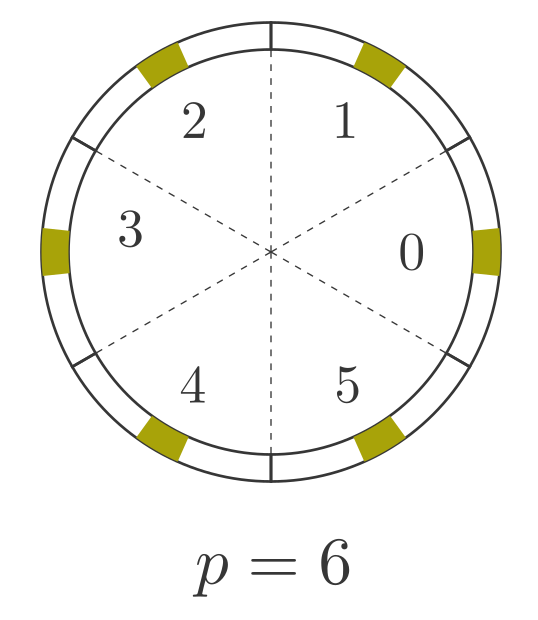
\includegraphics[width=0.5\linewidth]{images/busy_sectors_2.png}
    \end{subfigure}\hspace{1em}% Adjust the margin width as needed
    \begin{subfigure}{0.49\linewidth}% Specify the width here
        \centering
        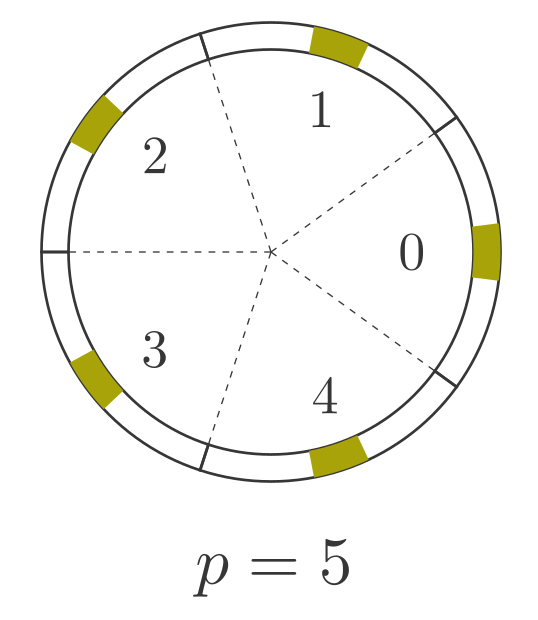
\includegraphics[width=0.5\linewidth]{images/busy_sectors.png}
    \end{subfigure}
    \caption{Distribution of the values of $\mu$ across $\Z_{q}$ for $p = 6$ and $p = 5$: the colored parts show the dense spots where the value has a high probability to lie in. The width of these sectors depends on $\sigma$ (the standard deviation of the error distribution $\chi$ of TFHE). Note that this repartition looks the same for $\Tilde{\mu}$ in $\Z_{2N}$.}    
    \label{fig:density_of_phase}
\end{figure}


When we transpose these dense spots into $\Z_{2N}$, they become the sectors close to $\left \{ \rounding{\frac{k \cdot 2N}{p}} \mid k \in \Z_p \right \}$. Let us note that the noises in $\Z_q$ and $\Z_{2N}$ are fundamentally different: the former is the one added at encryption that may have grew during the homomorphic computations, and the latter is called ``drift'' and is caused by the accumulation of the rounding errors on each coefficient of the ciphertext during the modulus switching (but this difference in nature does not impact our purpose). 
Let $k \in \Z_p$, the multiplication $X^{- \frac{k \cdot 2N}{p}} \cdot v(X)$ yields the same degree-zero coefficient as the multiplication  $X^{\modulo{- \frac{k \cdot 2N}{p} + N}{2N}} \cdot v(X)$, up to the minus sign. For the sake of clarity, we write the exponent of the latter in a slightly different manner: 
\[\modulo{
    \frac{
        -k \cdot 2N
        }
    {
        p
    }
    + N
}{2N} = 
\modulo{
    \frac{
    (-k + \frac p 2 ) \cdot 2N
    }
    {p}
}
{2N}\]


This is where the parity of $p$ plays a part: if $p$ is even, then $\modulo{
    \frac{
    (-k + \frac p 2 ) \cdot 2N
    }
    {p}
}
{2N}$ is a dense spot as well. So, the rotations by these two values will happen with high probability and they will both yield the same coefficient $v_{\frac{k \cdot 2N}{p}}$ (up to the minus sign for one of them). Thus, when evaluating a function $f$ with a PBS, the calls $f(k)$ and $f(k + \frac p 2)$ will produce the same output (one again, up to the minus sign), which is a collision constraining the definition of $f$. On the other hand, let us consider an odd value for $p$. Then, $\modulo{
    \frac{
    (-k + \frac p 2 ) \cdot 2N
    }
    {p}
}{2N}$ is no longer a dense spot, as it lies exactly halfway between the two dense spots $\modulo{
    \frac{
    (-k + \frac {p-1} {2} ) \cdot 2N
    }
    {p}
}{2N}$ and $\modulo{
    \frac{
    (-k + \frac {p+1} {2} ) \cdot 2N
    }
    {p}
}{2N}$. As a consequence, collision never occurs. Figure \ref{fig:torus_p_even_vs_odd} illustrates this phenomenon.


\begin{figure}
  \begin{subfigure}{0.49\linewidth}
    \    \centering
    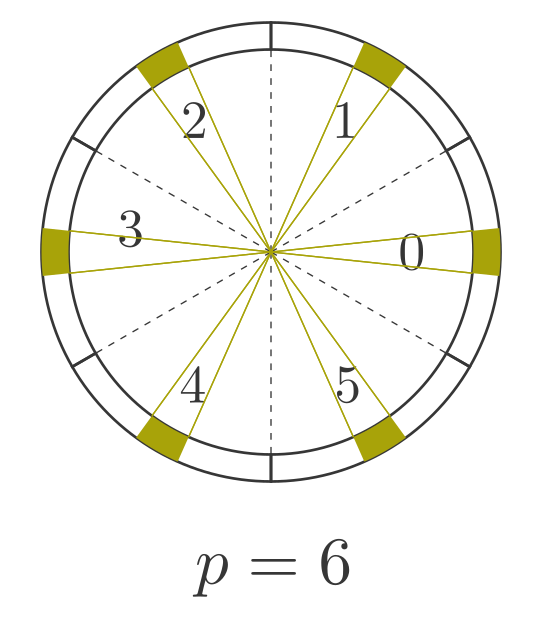
\includegraphics[width=0.5\linewidth]{images/torus_p_even.png}
    \caption{With $p$ even, the dense spots of each half of the torus are aligned.}
    \label{fig:torus_p_even}
  \end{subfigure}\hspace{1em}% Adjust the margin width as needed
  \begin{subfigure}{0.49\linewidth}
    \centering
    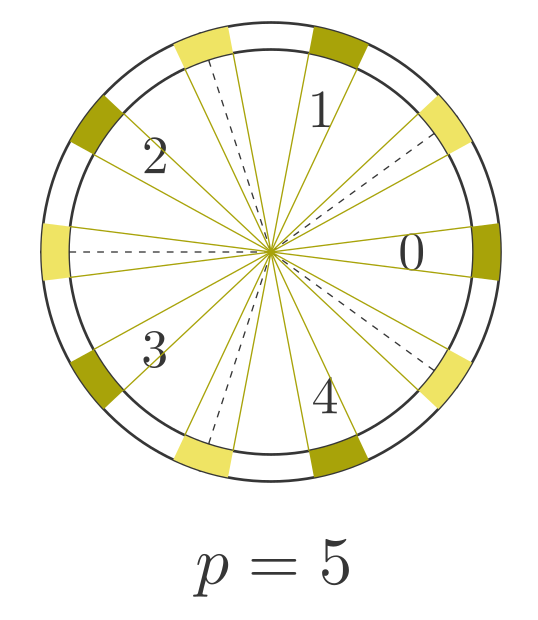
\includegraphics[width=0.5\linewidth]{images/torus_p_odd.png}
    \caption{With $p$ odd, the dense spots face empty spots, close to the bounds of the $p$-sectors.}
  \end{subfigure}
  \caption{}
  \label{fig:torus_p_even_vs_odd}
\end{figure}



That is why we select only odd values for $p$ in our framework. We will see in Section \ref{sec:parametrization} how this change impacts the parametrization of the scheme.



\paragraph{Exception for $p=2$:} We just said that only odd values can be selected for $p$ in our framework, however $p$-encodings with even values of $p$ exist as well: nonetheless they need to achieve the relaxed negacyclicity property introduced in Definition \ref{def:encoding}. This restriction makes them basically useless, as using only odd $p$-encodings is sufficient to evaluate all possible Boolean functions without having to bother with the negacyclicity property. However, the case $p=2$ is an exception: the valid $2$-encodings are automatically negacyclic and allow to evaluate the \texttt{XOR} operation by simply performing an homomorphic sum (so without bootstrapping). So it might be efficient to switch between $2$-encodings for \texttt{XOR} operations and $p$-encodings (with odd $p$) for non-linear Boolean functions. We make use of this strategy in our implementation of the Keccak permutation in Section \ref{sec:keccak} and for the AES in Section \ref{sec:aes}.



\subsection{Construction of the Accumulator for an Odd $p$}
\label{sec:accumulator}


The accumulator is the polynomial $v(X)$ used in the \texttt{BlindRotate} step of the PBS. In the Section \ref{sec:solving_negacyclicity}, we showed how the values are spread over the torus after bootstrapping. To actually make that works, we need to explicitly characterize this polynomial. In the following presentation, we neglect roundings to keep notations light (as if $p$ would divide $N$), or, equivalently, the division operator is assumed to include rounding.

\begin{definition}
    If $p$ is an odd modulus, and $f: \Z_p \mapsto \Z_{p'}$ a function, then the accumulator $v(X) \in \Z_{N, q}[X]/(X^N+1)$ has the form:\[v(X) = X^{- \frac {N} {2p}} \cdot \sum_{j=0}^{N/p - 1} X^j  \cdot \left ( \sum_{i=0}^{\frac{p-1}{2}} f(i) X^{i \frac{2N}{p}} + \sum_{i=0}^{\frac{p-1}{2} - 1} -f \left (i + \frac{p+1}{2} \right ) X^{i \frac{2N}{p} + \frac N p} \right )\]
\end{definition}


Let us explain the structure of this accumulator. The polynomial has degree $N$ and is made of $p$ distinct windows of width $\frac{N}{p}$. Each of these windows has constant coefficient value $f(k)$, for $k \in \{0, \dots, p-1\}$.
For $0 \le \alpha \le \frac{p-1}{2}$, the range of degrees whose coefficients are $f(\alpha)$ is $\left [ \alpha \frac{2N}{p} - \frac{N}{2p}~;~ \alpha \frac{2N}{p} + \frac{N}{2p} \right ]$. Now, for $\frac{p+1}{2} \le \beta \le p-1$, we can write $\beta = \alpha + \frac{p+1}{2}$, with $0 \le \alpha < \frac{p-1}{2}$. This time, the range of spanned degrees is $\left [ \alpha \frac{2N}{p} + \frac{N}{2p} ~;~ (\alpha + 1) \frac{2N}{p} - \frac{N}{2p} \right ]$. Thus, the values $k \in \{0, \dots, p-1\}$ spans the entire space $[0; N)$ without overlap. The values over $\frac{p+1}{2}$ gets negated by the negacyclicity, so the underlying coefficient is also negated to compensate this effect. We illustrate this construction on Figure \ref{fig:accumulator}.

\begin{figure}
    \centering
    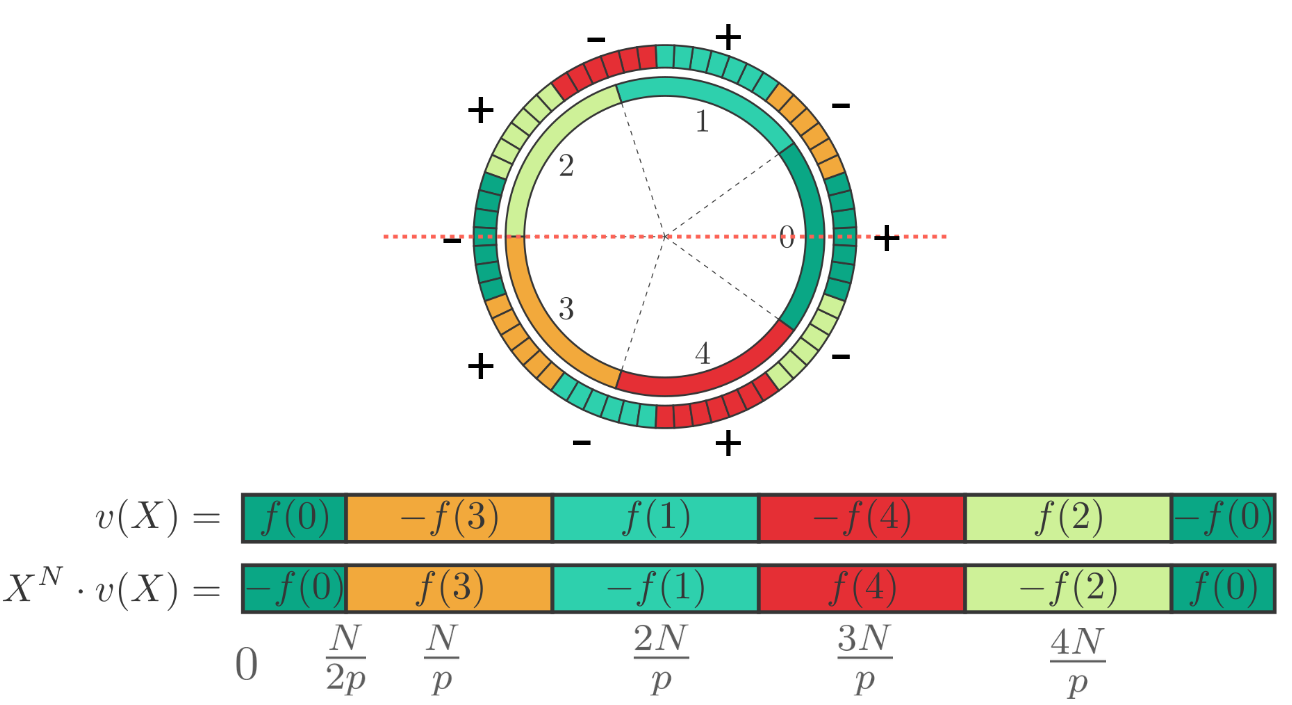
\includegraphics[width=\textwidth]{images/accumulator.png}
    \caption{Illustration of the construction of the accumulator. On top is the ring $\Z_{2N}$ splitted in windows. Below is a representation of the polynomial $v$, with its version once rotated by a multiplication by $X^N$. On the figure, $p$ = 5.}
    \label{fig:accumulator}
\end{figure}



\subsection{Crafting of Parameters}
\label{sec:parametrization}
The instances of the TFHE scheme are defined by a set of parameters. These parameters should simultaneously ensure the security of the scheme and the correctness of the homomorphic computations. They also determine the time of execution of one PBS. Here we define a framework to dimension the parameters required to optimally execute a given gadget.

Finding an optimal set of parameters for a given application is a hard problem and has been studied in particular in \cite{zama_parameters_optimization}. The parameters need to ensure three properties: security, correctness and efficiency. 

Let us start by an overview of the different parameters at play in an instance of the TFHE bootstrapping:

\begin{itemize}
    \item $n$: the dimension of the \LWE samples. Namely, the TLWE ciphertexts are vectors of length $n + 1$.
    \item $q$: the modulus of the ring the encrypted values live on. In \texttt{tfhe-rs} those values are stored on \texttt{u32} values, making $q = 2^{32}$. We treat this as an immutable platform-dependent value.
    \item $\sigma$: the standard deviation of the Gaussian distribution of error in \LWE samples.
    \item $k$: the dimension of the \GLWE samples. If $k=1$, we talk about \RLWE samples.
    \item $\sigma'$: the standard deviation of the Gaussian distribution of error in \GLWE samples.
    \item A few more parameters dimensioning some inner algorithms of the bootstrapping. A detailed description and an analysis of their impact on performances and noise level can be found in \cite{zama_parameters_optimization}. In this work, they are denoted as \emph{micro-parameters}.
\end{itemize}

In \cite{zama_parameters_optimization}, authors elaborate a strategy where they define an \textit{atomic pattern} of FHE operators, that is to say a subgraph of FHE operators in which the noise of the output is independent from the one in the inputs. Then, they develop an optimization framework to derive the best set of parameters for a given atomic pattern.

In particular, the first atomic pattern they study, that they denote by $\mathcal{A}^{(CJP21)}$, is a subgraph composed of a linear combination of ciphertexts with clear constants, then a \texttt{Keyswitch} and then a \texttt{BlindRotate} followed by a \texttt{SampleExtract} (\texttt{ModulusSwitch} is seen as a part of \texttt{BlindRotate}). Note that in Section \ref{sec:bootstrapping} we introduced the bootstrapping of TFHE by putting the \texttt{BlindRotate} before the \texttt{Keyswitch}, but the other way around is also doable. To dimension the parameters of TFHE to evaluate such an atomic pattern, their framework takes as input the 2-norm of the vector of constants of the linear combination (denoted by $\nu$) and a noise bound $t$ on the standard deviation of the distribution of error in a ciphertext that ensures a correct decryption with a good probability $(1-\epsilon$). We elaborate further on how this bound is constructed below in this section.

If we look closely, the evaluation of a gadget we introduced in Definition \ref{def:gadget} can be seen as a $\mathcal{A}^{(CJP21)}$ with a few differences. Thus, we slightly modified the tool \texttt{concrete-optimizer} \cite{concrete-optimizer}, that allows to generate parameters for different types of atomic patterns, to support our gadget as a new atomic pattern. Let us dive into the differences between a gadget and a $\mathcal{A}^{(CJP21)}$:

\paragraph{Support of odd values for $p$:} Using an odd value for $p$ changes the bootstrapping procedure, and in particular the definition of the accumulator for the \texttt{BlindRotate} (as explained in Section \ref{sec:accumulator}). With our construction, the windows in the polynomial are half the size of the ones for an even $p$, which impacts the noise bound $t$. 
As this bound depends of the failure probability $\alpha$ that the user is ready to tolerate, we shall denote it $t_\alpha$ hereafter, which satisfies: $t_\alpha = \frac{\Delta}{2z^*(1-\sqrt[N]{1-\alpha})}$
where $z^*$ is the \emph{standard score} and $\Delta$ is the scaling factor (see~\cite{zama_parameters_optimization} for more explanations). The impact of our adaptation on this formula is solely with respect to the scaling factor. In the context of an $\mathcal{A}^{(CJP21)}$, we have $\Delta = \frac{q}{2^\pi p}$ with $\pi$ the number of MSB for padding. As explained in Section \ref{sec:solving_negacyclicity}, we do not need any padding mechanism anymore, so the $2^\pi$ vanishes. However, the length of a window is divided by $2$, and $p$ does not divide $q$ anymore so we need to add a rounding. We finally get $\Delta = \rounding{\frac{q}{2p}}$.


\paragraph{Link between input encodings and $\nu$:} In a scenario where only one gadget has to be evaluated, its inputs are freshly encrypted ciphertexts. Then, there is no need to perform any encoding switching before evaluating the gadget, and so we are in the context of a $\mathcal{A}^{(CJP21)}$ with $\nu = 1$. However, if we are in a context of a \textit{graph} of gadgets like in Section \ref{sec:graphs}, the output of a gadget can be used as input of subsequent gadgets under different encodings. In this case, some encoding switchings are necessary. If these encoding switching are made using a mutiplication by a constant (Property \ref{prop:mult_constant}), we are still in the context of a $\mathcal{A}^{CJP21}$ but with $\nu \ne 1$. 
To formalize that, we first recall that Algorithm \ref{alg:add_element} produces gadgets of the form $\Gamma = \left (\vec{\Encoding_{in}}, \Encoding_{out}, p_{in}, p_{out}, f \right )$, with $\Encoding_{in}^{(i)} = \EncDefOne{d_i}$. Thus, if we fix that all gadget output ciphertexts are encoded under $\Encoding_{out} = \EncDefOne{1}$, then the encoding switchings needed before an evaluation of $\Gamma$ corresponds to a linear combination of the inputs with the vector $\vec d = (d_i \mid i \in [1, \ell])$, so we fall back on a $\mathcal{A}^{(CJP21)}$ with $\nu = \customnorm{\vec d}$.


We implemented these changes in \texttt{concrete-optimizer} and uses it to generate sets of parameters for our implementations detailed in Section \ref{sec:implementations}.

\subsection{Concrete Implementations of $p$-Encodings and Homomorphic Functions in \texttt{tfhe-rs}}
\label{sec:library}


To implement our framework, we relied on the $\texttt{tfhe-rs}$ library~\cite{tfhe-rs}. Here is a list of the major changes we applied to the code:

\paragraph{Addition of the notion of $p$-encoding: } An encoding $\Encoding$ is simply implemented with a structure \texttt{Encoding} storing two \texttt{HashSets} and the modulus $p$. The \texttt{HashSets} represent both sets $\Encoding(0)$ and $\Encoding(1)$. When creating an \texttt{Encoding}, the code checks whether the two underlying sets are disjoint or not. Moreover, the operation of encryption and decryption are modified as well. The signatures change from:\[\texttt{encrypt(Boolean, ClientKey) -> Ciphertext}\] to: \[\texttt{encrypt(Boolean, ClientKey, Encoding) -> Ciphertext}\] (same for \texttt{decrypt}). The functions also perform the mapping $\B \mapsto \Z_p$ before encryption and the other way around after decryption.


\paragraph{Support of odd moduli: } The native \texttt{tfhe-rs} only support power-of-two-moduli $p$. We extended the library to handle odd values for $p$. This required modifying the encryption and decryption algorithm, and to compute the sets of parameters with the method of Section \ref{sec:parametrization}.


\paragraph{Definition of the new structure $\texttt{Gadget}$: } According to the evaluation strategy we introduced in Section \ref{sec:new_strategy}, we wrote a new structure $\texttt{Gadget}$, associated to a Boolean function $f: \B^\ell \mapsto \B$, carrying:
\begin{itemize}
    \item A list of the \texttt{Encoding} objects for the inputs: $\Encoding_{in} = (\Encoding_1, \dots, \Encoding_l)$, with the input modulus $p_{in}$ they encoded on.
    \item The output \texttt{Encoding} object $\Encoding_{out}$, with the output modulus $p_{out}$ it is encoded on.
    \item The clear function $f$.
\end{itemize}
When such a structure is constructed, it self-checks whether $f(\Encoding_{in})$ is valid. Then, when provided $\ell$ $\texttt{Ciphertexts}$ objects encoded under their respective $p$-encoding, it executes the homomorphic sum and the PBS and outputs the results encoded under $\Encoding_{out}$. Some utilitary functions performing encoding-switching are also available, allowing the chaining of several $\texttt{Gadget}$.


\paragraph{Implementation of the accumulator: } The procedure of bootstrapping of \texttt{tfhe-rs} is slightly modified to support the new version of the accumulator we introduced in Section \ref{sec:accumulator}.

\paragraph{Parsing of graphs: } We implemented a Python script that produces graphs to represent more complex functions that requires several PBS, as described in Section \ref{sec:graphs}. These graphs are stored with a comprehensive file format and our Rust implementation has a module of parsing allowing to load these graphs and automatically generate the corresponding graph of \texttt{Gadget}.



